\documentclass{article}
\usepackage{pgfplots}
\pgfplotsset{compat=1.17}
\usepackage{tikz}
\usetikzlibrary{shadings, decorations.pathmorphing}
\usetikzlibrary{backgrounds,
                hobby}
\begin{document}

\begin{figure}
    \centering
    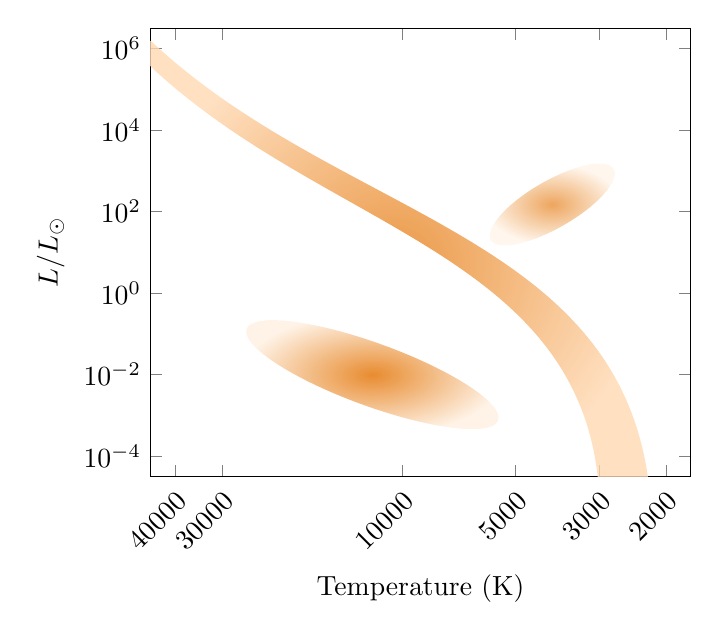
\begin{tikzpicture}[
        ban/.style={fill=orange!80, draw=none},
    ]
        \begin{loglogaxis}[
            xlabel={Temperature (K)},
            ylabel={$L/L_\odot$},
            xmin=2000, xmax=40000,
            ymin=1e-4, ymax=1e6,
            xtick={2000, 3000, 5000, 10000, 30000, 40000},
            xticklabels={2000, 3000, 5000, 10000, 30000, 40000},
            ytick={1e-4, 1e-2, 1, 1e2, 1e4, 1e6},
            x dir=reverse, % Reverse the x-axis for Temperature
            %grid=both,
            minor tick num=5,
            major grid style={black!50},
            minor grid style={gray!25},
            xticklabel style={anchor=north east, rotate=45}, % Slant the labels
            enlargelimits={0.05}, % //Adds 10% extra space
            ]


            % White dwarfs region with a fuzzy oval
            \shade[inner color=orange!80!gray, outer color=orange!10!white, opacity=0.9]    
                        (12000, 1e-2) ellipse [x radius=1.7cm, y radius=0.4cm, rotate=-20]; % Inner bright part
                          
            % Giants region with a fuzzy oval
            \shade[inner color=orange!80!gray, outer color=orange!10!white, opacity=0.7]    
                        (4000, 1.5e2) ellipse [x radius=0.9cm, y radius=0.3cm, rotate=30]; % Inner bright part
                       
                                
             % ~~~ the 4th region ~~~~~~~~~~~~
           \shadedraw[
                inner color=orange!80!gray, 
                outer color=orange!30!white, 
                opacity=0.8,
                draw=none
              ]            
                    (axis cs:50000,7e5) to[out=-45,in=93] 
                    (axis cs:3000, 1e-5) --
                    (axis cs:2200,1e-5) to[out=95,in=-45] 
                    (axis cs:50000, 3e6) -- cycle;
       
                
 % Thinner shape by scaling the y-axis
    %        \scoped[on background layer, yscale=0.3]{ % Apply vertical scaling
    %            \path[use Hobby shortcut, closed=true, inner color=orange!80]
    %            (20000, 9.9e18)  
    %            .. (10000, 1e20)   
    %            .. (3000, 1e20)    
    %            .. (3000, 9.9e18)    
    %            .. (20000, 9.9e18);  
    %        }

      
  \end{loglogaxis}
    \end{tikzpicture}
    \caption{Hertzsprung-Russell Diagram with Supergiants Region (Banana Shape)}
\end{figure}


\end{document}